\documentclass[10pt,a4paper]{article}
\usepackage[margin=18mm]{geometry}
\usepackage[T1]{fontenc}
\usepackage{lmodern,amsmath,amssymb,booktabs,array,graphicx,xcolor,hyperref}
\hypersetup{colorlinks=true,urlcolor=blue,linkcolor=blue}
\setlength{\parindent}{0pt}
\setlength{\parskip}{5pt}
\pagestyle{plain}
\newcommand{\F}{\mathbb F}
\newcommand{\code}[1]{\texttt{#1}}
\begin{document}
\begin{center}
{\LARGE Actual twist useful yield and S3 degrees}\\[5pt]
{\large A finite positive example, its scalar reduction, and its pullback control}\\[4pt]
2026-10-24 \quad \code{s3-yield-20261024} \quad PR \#2381
\end{center}

An actual twist factor base gives two independent rows at a public relation
target where the main curve's prefix base gives none. Its finite Macaulay
closure degree is4 instead of6. An explicit base-field map preserves the
unknown scalar. \textbf{The same gain is reproduced by pulling the factor base
back to the main curve; homogeneous regularity is equal. No speedup is measured.}

Over $\F_{43}$ use $E:y^2=x^3+x$, $T:Y^2=X^3+4X$, nonsquare twist
parameter $d=2$, $r=11$, $P=(31,18)$ and $U=(24,26)$. Both rational groups
have order44. The model IDs are \code{icv1-fp6-t0-74779950} and
\code{icv1-fp6-t0-c6a8a47c}. The frozen policy selects the first two subgroup
x coordinates, with the least y representative at each x.

\begin{center}\small
\begin{tabular}{@{}p{74mm}rr@{}}\toprule
First public precomputation target & Main & Twist\\\midrule
Base points & $(4,5),(13,19)$ & $(15,9),(17,6)$\\
Ordered S3 root pairs out of four &0&3\\
Distinct accepted rows mod11 &0&2\\
Independent row gain &0&2\\
Finite vanishing-space closure degree &6&4\\
First refutation degree &5& absent\\
Leading-ideal first-zero degree &3&3\\\bottomrule
\end{tabular}\end{center}

Writing $B_0=(15,9)$, $B_1=(17,6)$, the actual twist point relations are
$B_0+B_1=U$ and $-(B_0+B_0)=U$. Their log equations are
$\ell_0+\ell_1=1$, $-2\ell_0=1\pmod {11}$, with nonzero determinant $-2$;
they uniquely give $(\ell_0,\ell_1)=(5,7)$. Lean checks these on actual
Mathlib nonsingular points and checks that the main prefix base has no such
signed decomposition at $P$.

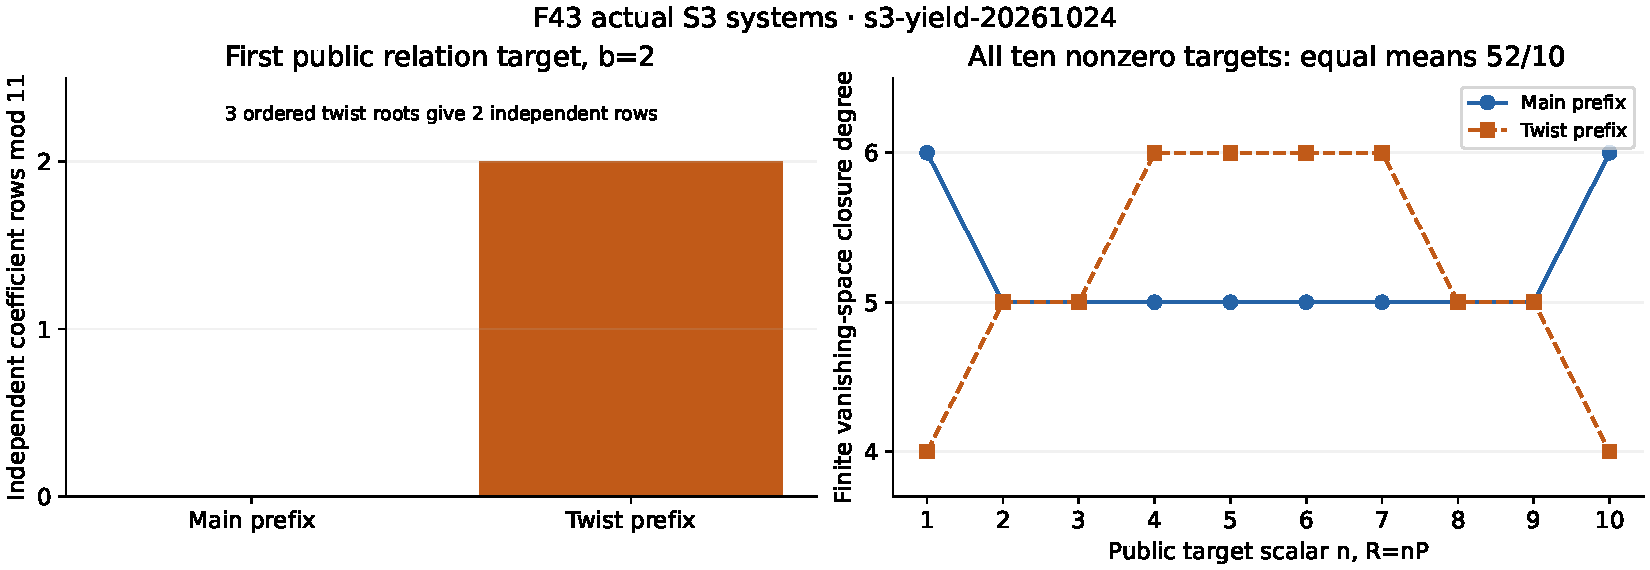
\includegraphics[width=\linewidth]{profiles.pdf}
{\footnotesize Recorded native values, independently replayed. The right panel
contains every nonzero target: both closure sums are52 over ten targets.
The left panel counts independent rows, not a probability or a timing.}

\newpage
{\Large The actual equations and three different degree notions}

For each nonzero subgroup target $R=nP$, $n=1,\ldots,r-1$, the exact
prime-field system is
\[
 S_{3,a,b}(x,y,x(R))=0,\qquad g_B(x)=g_B(y)=0,
 \quad g_B(t)=\prod_{u\in B_x}(t-u).
\]
Here
\[
 S_{3,a,b}(x,y,z)=(x-y)^2z^2
 -2\big((x+y)(xy+a)+2b\big)z+(xy-a)^2-4b(x+y).
\]
Every root pair is lifted to actual signed point relations. Repeated x values
are included. No unperformed Weil-descent or rationality system replaces these inputs.

\textbf{Homogeneous leading ideal.} For fixed z, the degree4 component of S3
is exactly $x^2y^2$. For a monic base polynomial of size $b=2$ or3, the leading
components are $x^b,y^b$. Lean proves the actual leading-form ideal is
\[
 I_{\rm top}=\langle x^2y^2,x^b,y^b\rangle,
\]
independent of curve coefficients, target and base locations. Its standard
monomials satisfy $i<b$, $j<b$ and $(i<2\ \text{or}\ j<2)$. A degree-b
monomial survives, and none survives degree $b+1$. Native Hilbert vectors are
$[1,2,1,0,0]$ for b2 and $[1,2,3,2,0,0]$ for b3.
The first-empty degrees3 and4 are the homogeneous degree-of-regularity
convention used here. \textbf{They do not decrease under this twist comparison.}
They are not equated to F4/F5 runtime, solving degree or the quotient's
Castelnuovo--Mumford regularity.

\textbf{Finite closure degree.} At each $D=\max(4,b),\ldots,12$, build every
monomial multiple of each input of total degree at most D. Let $M_D$ be their
coefficient row space and $\operatorname{ev}_D$ evaluation on every actual root.
The recorded criterion
\[
 \dim M_D+\operatorname{rank}(\operatorname{ev}_D)=\dim V_D
\]
certifies $M_D=\ker(\operatorname{ev}_D)$, since every row vanishes at the roots.
This is the labelled finite vanishing-space closure degree, not an asserted
F4/F5 degree. Every tested system closes by the cap.

\begin{center}\small
\begin{tabular}{lrrrrl}\toprule
First target &D&columns&$\dim M_D$&eval rank&unit derived?\\\midrule
Main &4&15&12&0&no\\
Main &5&21&20&0&yes\\
Main &6&28&28&0&yes; closure\\
Twist &4&15&12&3&no; closure\\\bottomrule
\end{tabular}\end{center}

\textbf{Refutation degree.} A Lean-checked explicit dual functional kills all
thirteen main degree4 input multiples but sends1 to1; hence no degree4
refutation exists in this filtration. An explicit degree5 combination derives1.
Thus the first refutation degree is5; closure6 is the stronger criterion.
The twist has three actual roots. Its degree4 closure is independently checked
by native matrix replay; no lower homogeneous regularity is inferred.

\newpage
{\Large Verified source reduction and the decisive control}

The base-field map
\[
 \phi(O)=O,\qquad \phi(x,y)=(41x,11y)
\]
is an actual injective additive map $E(\F_{43})\to T(\F_{43})$, with $\phi(P)=U$.
Lean proves for arbitrary actual points A,B and integer n:
\[
 \phi(B)=n\phi(A)\quad\Longleftrightarrow\quad B=nA.
\]
No logarithm table defines this map. This is an exceptional j1728, trace-zero
quadratic twist which is also base-field isomorphic; the map is not asserted
for arbitrary or ordinary twists.

\begin{center}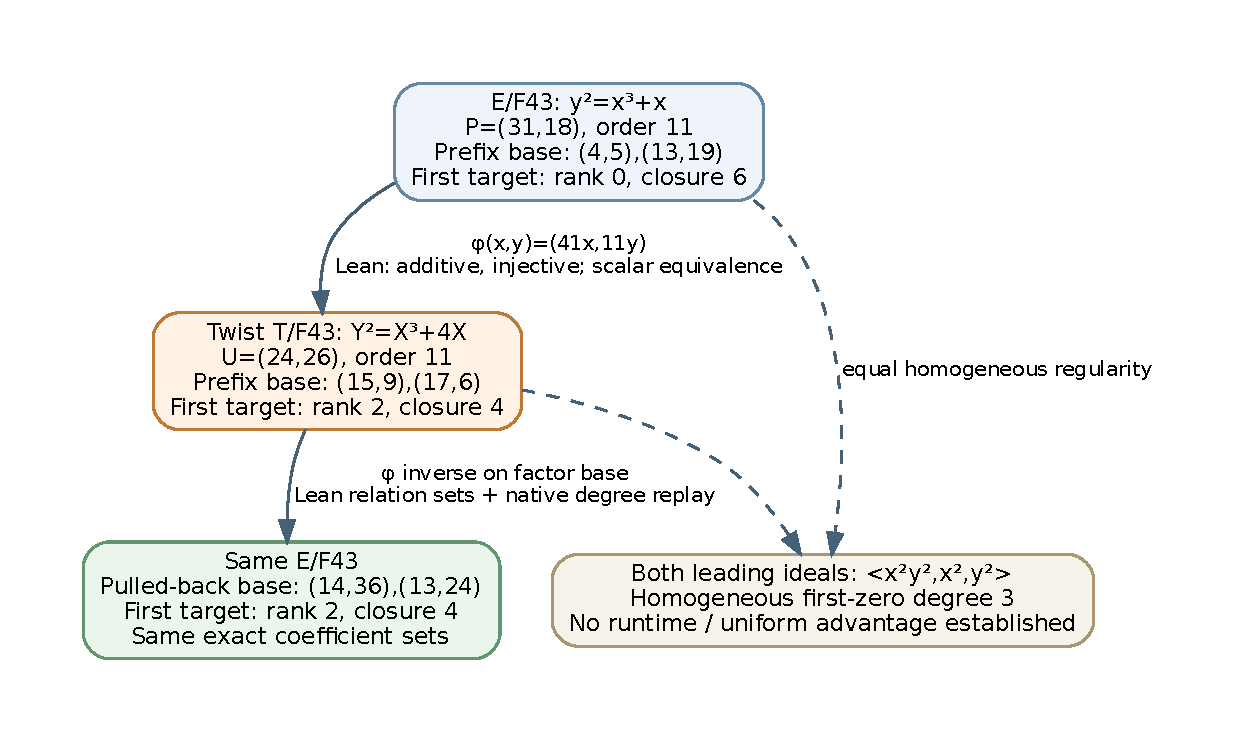
\includegraphics[width=\linewidth,height=89mm,keepaspectratio]{bridge.pdf}\end{center}

Pulling back the twist base gives main points $(14,36),(13,24)$. Lean checks
their images and both relations at P. It proves equality of the entire
accepted coefficient sets for every finite integer candidate set, with the
target included as a third column. Native replay reproduces every coefficient
row, rank state and matrix-degree profile in both transport directions.
\textbf{The finite advantage therefore can be realized as factor-base choice
on the original main curve.}

The explicit native precomputation checks sixteen signed ordered candidates
per target. Main and twist bases reach two independent rows after three and
one complete public targets respectively: two rows from48 versus16 signed
candidates. Those are finite batch counts. A PDP call can emit multiple rows;
two rows per call is not a probability of two. The prior positive-yield cost
theorem is not instantiated using a fictitious positive main yield at the
first target, where it is zero.

Across all ten nonzero targets, both arms finish at rank2 and mean closure
degree $52/10=5.2$. The twist loses on closure degree at targets4--7. All twenty
size2/size3 subset policies, including ties and losses, are retained. Six have
both greater first-target rank and lower closure; only one improves rank after
the first three targets.

The independent Rust toy IC solver constructs relations without reading the
recorded scalar labels, solves the base-log matrix, and recovers all eleven
synthetic main targets after mapping, using lookup or signed-pair descent with
explicit shifts. Independent scalar checks pass. These are separate correctness
cases, not one-target timing or amortized throughput. Setup, transfer, failures,
linear algebra, descent and verification still need matched cost accounting.

\newpage
{\Large Evidence, proof scope and remaining goal}

\begin{center}\small
\begin{tabular}{@{}p{92mm}r@{}}\toprule
Finite coverage / validation &Result\\\midrule
Original short models, p5,7,11,13,17,19 &942\\
Shared odd-prime cases / r3 too small for two x points &274 /186\\
Eligible cases / primary size2,size3 comparisons &88 /104\\
Additional F43 subset comparisons &20\\
All comparisons / target systems including controls &124 /1,904\\
Transported / inverse-transported target controls &272 /272\\
Strictly lower homogeneous first-empty degree &0\\
Named study theorems / audited declarations &144 /185\\
Extra trusted axioms / failing declarations &0 /0\\
Release library tests passed / existing ignores &4,479 /119\\
Isolated native backend / workflow metadata tests &22 /4\\\bottomrule
\end{tabular}\end{center}

The C++ producer reuses unchanged field/curve arithmetic. Rust independently
enumerates points with a linear addition chain, constructs S3 using a separate
coefficient table and symmetric evaluation, and uses batch RREF with a different
monomial order. C++ uses incremental echelon insertion. Rehashed false-rank,
false-degree, missing-case and false-scaling payloads reject exit101 without
receipts. All failures and provisional runs remain in the validation archive.
The first library test run's nine loopback socket denials are preserved; the
network-enabled full rerun passes, with no source/test patch or skipped case.

Lean4.34.1 / Mathlib \code{d13f23b723b8a846827a245b89c10fc7d3f11612} remain pinned.
The unmodified gate passes twelve modules. The41 other audited declarations
include generated helpers; only propext, Classical.choice and Quot.sound occur.
No trusted native evaluation or external lean4checker replay is claimed.

{\small\begin{tabular}{@{}p{46mm}>{\raggedright\arraybackslash}p{116mm}@{}}
Leading forms and actual ideals &\code{S3System.s3\_leading\_component}, \code{size2\_leading\_ideal}, \code{size3\_leading\_ideal}, \code{actual\_head\_ideal\_cutoff}\\
Actual scalar reduction &\code{S3System.F43.scalar\_reduction}\\
Actual useful relations &\code{S3System.F43.twist\_first\_relation}, \code{twist\_second\_relation}, \code{recovered\_base\_logs}\\
Degree certificates &\code{S3DegreeFixture.no\_degree4\_refutation}, \code{degree5\_unit\_certificate}\\
Pullback equality &\code{S3DegreeFixture.pulled\_back\_relation\_sets}
\end{tabular}}

Two source-bound polynomial certificates each pass32+16 native points and
false-plus-one/source controls:
\begin{quote}\small
\code{IDC1hf15c17737ed713d5}: S3 scaling.\\
\code{IDC1hcee4710ff9dcf7e7}: cleared degree5 unit identity.
\end{quote}
Lean separately
checks characteristic43, the dual, actual points and maps. All prior ten
certificates, frozen sources and reports remain unchanged.

\textbf{Status.} The finite useful-row/closure example and actual F43 DLP
reduction are verified. Strict homogeneous regularity improvement is refuted
for this encoding. Uniform useful yield, a lower relevant degree for another
encoding, compatible complete work bounds and practical advantage remain open.
The next requirement is an actual encoding whose leading ideal can change,
with a verified subgroup reduction and a pullback control. It is not a running job.

The new twist generator is recorded explicitly; its old registered EC1 uses
$(35,12)$, not $(24,26)$, and is not reused. No registry, leaderboard, cover or
conflicted claim input changes. General geometry, exact-head CI/review,
merge/integration and shared Conductor gates remain; Conductor exits127 and
no reservation or replacement coordinator is claimed. No hardness, GHS,
invalid-curve attack or speed claim is made.

{\footnotesize Sources and reproduction: protocol \code{S3\_YIELD\_20261024\_PROTOCOL.md};
\code{native/s3-yield-20261024/}; \code{validation/s3-yield-20261024/};
new Lean modules and the pinned Mathlib homogeneous-polynomial/ideal and
elliptic-point APIs. Run the unchanged proof gate and \code{run-s3-yield.sh}
from the repository root. Full paths, checksums, exact commands, raw controls
and scope limits are in the accompanying README.}
\end{document}
